
\chapter{Math Load Model}

The previous chapter described the major background, necessary for the rest of this work. As shown in the introduction, very few progress was observed in the CO formulation. This chapter proposes new constraints and strategies for expanding the CO model. We are especially interested in constraints for modeling the signature of a load and improve its performance. First, the classic NILM optimization problem is reformulated as a MILP problem. Then, three constraints are proposed for defining a load signature such as the transition of states and minimum time. Strategies and constraints for decreasing the computation time are also introduced. Finally, the full proposed model is presented. 

\section{Mixed-Integer Linear Programming (MILP) Formulation}

The CO formulation in the Equation \eqref{classic2} can be reformulated as a MILP problem, shown in \eqref{milp2}--\eqref{eq7}. This way, the new formulation becomes suitable to linear solvers.

\begin{equation} \label{milp2}
    \min_{x_i(t)} \quad \sum_{t\ \in\ T} \delta_P(t) + \delta_Q(t)
\end{equation}

subject to 

\begin{equation} \label{eq65}
    P(t) - \sum_{i\ = 1}^{n} x_i(t)\ P_i \ \leq \ \delta_P(t) 
\end{equation}

\begin{equation} 
  P(t) - \sum_{i = 1}^{n} x_i(t)\ P_i \ \geq \ -\delta_P(t)
\end{equation}

\begin{equation} 
   Q(t) - \sum_{i\ = 1}^{n} x_i(t)\ Q_i \ \leq \ \delta_Q(t)
\end{equation}

\begin{equation} \label{eq7}
  Q(t) - \sum_{i = 1}^{n} x_i(t)\ Q_i \ \geq \ -\delta_Q(t)
\end{equation}

Where $\delta_P(t)$ and $\delta_Q(t)$ in \eqref{milp2} are the errors in the active and reactive power. Those errors are defined as the difference between the aggregated power states and the actual measurement (i.e., the approximation error). Besides the linear formulation, another difference from \eqref{classic2} is that the time $T$ is included in the objective function. The advantage of doing this is the possibility of adding new time-dependent constraints in order to improve the model's accuracy. 

However, as previously discussed, this formulation has many limitations. One of them is the confusion of similar loads. The Figure \ref{image32} illustrates this problem. 


\begin{figure}[tb]
    \centering
    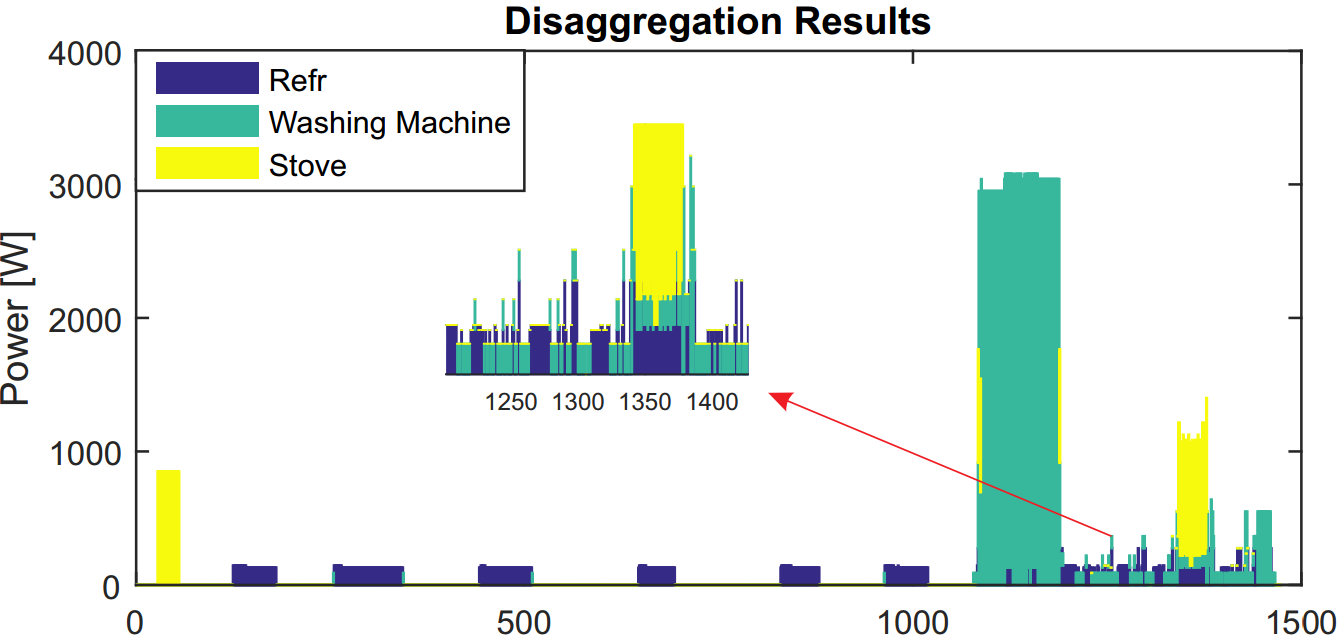
\includegraphics[width=1\columnwidth ]{image32.png}
    \caption{Illustration of the MS problem that occurs in the CO classic formulation}
    \label{image32}
\end{figure}





\section{Visual Intuition}
Before diving into equations, let's get some visual intuition on model that is going to be presented. First, let's imagine the disaggregation problem as puzzle where the goal is to find the best set of pieces to fit a given space. An example of this scenario is illustrated in the Figure~\ref{blocks}. 

\begin{figure}[tb]
    \centering
    
\includegraphics[width=1\columnwidth ]{blocks.png}
    \caption{Illustration of the problem with a puzzle}
    \label{blocks}
\end{figure}

First, a model for each of the pieces could be created. This model could consider the height and width of rectangular block. Next, more complex pieces could be created as a set of rectangular blocks, such as the purple block. Finally, in order to solve the puzzle, this scenario could be treated as a combinatorial problem. The goal would be to find the set of blocks that better fits in the gray space. 


The proposed NILM model of this work is somewhat similar the very same analogy. Now, the goal is to find the set of appliance's models that better fit in the whole aggregated power of a region. The only difference is that now a minimum width is defined, instead of a fixed width. As an example, the appliance model could be built from three parameters presented in the Figure~\ref{example}: 

\begin{itemize}
\item The minimum time $MD_i$ in which each state $i$ should remain ON.
\item The sequence of states of an appliance, defined by the parameter $\text{prev}_i$
\item The index of states for each appliance, given by $D_i$.
\end{itemize}

With those parameters, we can now introduce the constraints of the next section. 
\begin{figure}[htb]
    \centering
    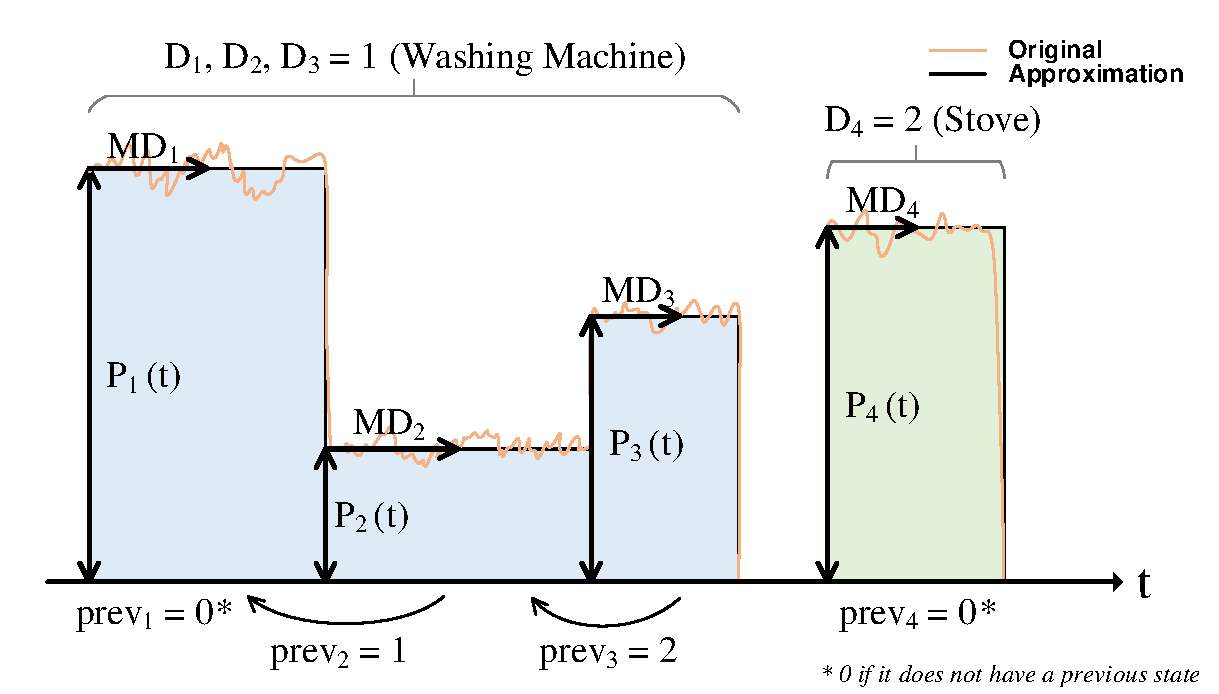
\includegraphics[width=1\columnwidth ]{example_2.pdf}
    \caption{Two hypothetical load signatures to be modeled}
    \label{example}
\end{figure}



\section{Load Signature Constraints}

In this section, a new set of constraints are presented to model the load signatures and to communicate the optimization process of one window with the others. First, let's consider a practical example. Fig.~\ref{example} shows the load signature of two hypothetical appliances: a washing machine and a stove.


The washing machine's load signature can be approximated using three power states ($P_1(t)$, $P_2(t)$ and $P_3(t)$) while the stove's has one single power state ($P_4(t)$). In order to model these loads, the following hypotheses are considered: 

\begin{itemize}

\item Multiple states $P_i(t)$ (also multiple reactive power states, if available) from the same appliance cannot be activated simultaneously;
\item Some loads work as finite-state machines, i.e., a given state is only activated if another state of the same appliance has finished;
\item A state $i$ can have a minimum time $MD_i$ in which it should remain ON.

\end{itemize}

The former hypotheses are used to formulate a set of constraints used to efficiently represent the load signatures within the proposed MILP model. A detailed analysis of each one of the former hypotheses is shown in the following subsections.

\subsection{Avoiding Multiple States From the Same Appliance}

Parameter $D_i$ identifies the appliance's index of each state $i$. For example, the states $i = 1, 2, 3$ in Fig.~\ref{example} are associated to the washing machine, that is, $D_1 = D_2 = D_3 = 1$, where the number 1 means ``washing machine''. Likewise, $D_4$ refers to the stove, identified by the number 2. In order to avoid simultaneously allocation of different power states from the same appliance, constraint \eqref{overl} can be included.

\begin{equation} \label{overl}
   \sum_{i \in S | D_{i} = j} x_i(t) \leq 1 \quad \forall t \in \tilde{T}, j \in D
\end{equation}

Constraint \eqref{overl} limits the sum of the states $x_i(t)$ from the same appliance to one. This way, $x_1(t)$, $x_2(t)$ or $x_3(t)$ cannot be simultaneously activated since $D_1$, $D_2$ and $D_3$ are associated to the same appliance.

\subsection{Linking the Transition Between Power States}

In Fig.~\ref{example}, power state $P_2(t)$ should be ON only if the power state $P_1(t)$ has finished. Likewise, we could also fix the power state $P_3(t)$ to be ON only if $P_2(t)$ has finished. The goal is to include a constraint that allows a specific power state to be activated only if a previous one (from the same appliance) has finished. To do so, two binary variables are used to determine the transition from a ON state to an OFF state, and vice versa. The two variables are called $up_i(t)$ (turned ON) and $dw_i(t)$ (turned OFF). Then, the linking constraints are given by \eqref{updw}--\eqref{updw2}.
%
%\vspace{-10pt}

\begin{equation} \label{updw}
    x_i(t) - x_i(t-1) = up_i(t) - dw_i(t) \quad \forall i \in S, t \in T
\end{equation}


\begin{equation} \label{updw2}
    up_i(t) + dw_i(t) \leq 1 \quad \forall i \in S, t \in T
\end{equation}

\noindent where $X_i$ saves the state $x_i(t)$ of the last time period of each window, necessary for the initialization of $x_i(t)$ in the next window. In constraint \eqref{updw}, $up_i(t)$ will be 1 only if the decision variable $x_i(t)$ makes a transition from 0 to 1, at time $t$. Likewise, $dw_i(t)$ will be 1 only if $x_i(t)$ makes a transition from 1 to 0, at time $t$. Next, \eqref{updw3} links the state transitions between windows. Finally, \eqref{updw2} prevents $up_i(t)$ and $dw_i(t)$ to be simultaneously 1.

%Now that we have these two variables, let's consider that we save the transition of states in a parameter called $\text{prev}_i$. In the Fig. \ref{example} we have for example in the washing machine that the value of $prev_2$ is 1 since we want to fix the second state to happen only after the first one. We can fix state transitions using the following constraint:

Using constraints \eqref{updw}--\eqref{updw2} and the parameter $\text{prev}_i$, we can now link the transition between two states using the additional equation in \eqref{state}.

\begin{equation} \label{state}
    up_i(t) = dw_{\text{prev}_i}(t) \quad \forall i \in S, t \in T \ | \ \text{prev}_i>0
\end{equation}

As an example, the state $i = 2$ of the washing machine in Fig.~\ref{example} can only change from OFF to ON (i.e., $up_2(t) = 1$) if the state $i = 1$ has change from ON to OFF (i.e., $dw_1 = 1$), at a given time $t$.

\subsection{Minimum Active Time}

One last hypothesis that is proposed in this paper is setting a minimum active time of a state. Parameter $MD_i$ in Fig.~\ref{example} establishes the minimum number of time samples in which the state $i$ should be kept activated. The set of constraints presented in \eqref{md1}--\eqref{md3} are proposed to carry out this process. 

\begin{multline}\label{md2}
    \sum_{k\ =\ t}^{t+MD_i-1} x_i(k) \geq MD_i \left[ x_i(t) - x_i(t-1) \right] \\
    \forall i \in S, t \in 2 \hdots |T| - {MD}_i + 1
\end{multline}

Where $|T|$ is the total number of samples, i.e., the last sample in $T$. Constraint \eqref{md1} activates a certain state that was already activated at the end of the previous window, but for less than $MD_i$ samples. Constraint \eqref{md2} forces $x_i(t)$ to be 1 for at least $MD_i$ time samples. Finally, constraint \eqref{md3} is used to represent the operation at the final portion of the window, when there are less than $MD_i$ samples available. It forces a given state $x_i(t)$ to be ON until the end of the window, only if it has been activated at any moment within this final interval. The size of $MD_i$ has as limit the length $m$ of the window, i.e, $MD_i \leq m$. 
As a side note, the set of equations presented in \eqref{overl}--\eqref{md3} are similar to models of the operation of thermal units in the unit commitment problem, proposed by authors in \cite{carrion2006}.

\section{Window-based formulation}
The time set $T$ increases the computational burden since the variable $x_i(t)$ depends on the number of time periods. To overcome this issue, it is possible to separate the set of time periods into smaller, homogeneous windows. Let $\tilde{T} \subset T$ be the set of time periods within a window, where $\tilde{T} = \left\{ T_{0} , T_{0} + 1, \cdots , T_{0} + m \right\}$, $m$ is the number of time steps of the window, and $T_{0}$ is the initial period for each window. The Figure \ref{windows} illustrates the separation of the time periods. The MILP problem can now be written using a sequenced  optimization process as shown in Algorithm \ref{algorithm1}, where $T_{\text{end}}$ is the final period of $T$.


\begin{figure}[tb]
    \centering
    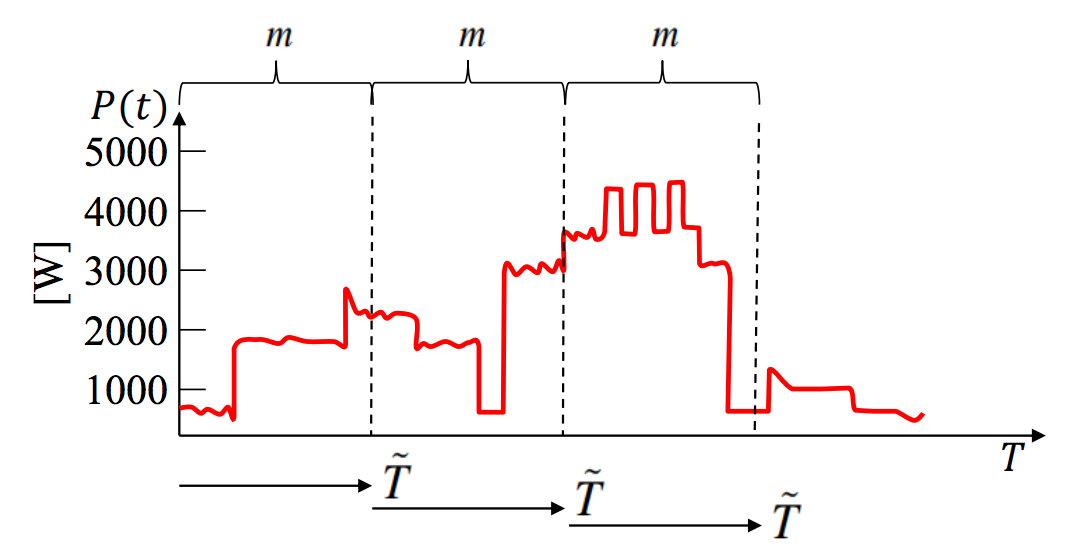
\includegraphics[width=1\columnwidth ]{windows.png}
    \caption{Tew time space in a window-based algorithm}
    \label{example}
\end{figure}


\begin{algorithm}\label{algorithm1}
\SetAlgoLined
 \Repeat{$T_{0}$ > $T_{\text{end}}$}{

let  $\tilde{T} = \left\{T_{0}, \cdots, T_{0}+m \right\}$

solve
\begin{equation}
    \min_{x_i(t)} \quad \sum_{t\ \in\ \tilde{T}} \delta_P(t) + \delta_Q(t)
\end{equation}

s.t.:

\begin{equation} \label{first_eq}
    P(t) - \sum_{i = 1}^{n} x_i(t)\ P_i \ \leq \ \delta_P(t)
\end{equation}

\begin{equation}
  P(t) - \sum_{i = 1}^{n} x_i(t)\ P_i \ \geq \ -\delta_P(t)
\end{equation}

\begin{equation} \label{third_eq}
    Q(t) - \sum_{i = 1}^{n} x_i(t)\ Q_i \ \leq \ \delta_Q(t)
\end{equation}

\begin{equation} \label{fourth_eq}
  Q(t) - \sum_{i = 1}^{n} x_i(t)\ Q_i \ \geq \ -\delta_Q(t)
\end{equation}


let $T_0 = T_0 +m +1$
 }
 \caption{NILM using a window-based algorithm}
\end{algorithm}

Algorithm 1 is still equivalent to the classic optimization formulation and will be used as one of the approaches to be compared in the results. 



One constraint that is helpful for cases in which the reading in the window is less than a given threshold (for example $TH = 30W$). The constraint \eqref{set_zero} allows to automatically set to zero the binary variables under those circumstances. 

\begin{equation} \label{set_zero}
   x_i(t) = 0 \quad \forall t \in \tilde{T}, i \in S | P(t) \leq TH
\end{equation}

The constraints for the transition between states and minimim active time have now to be adapted to the window based algorithm.

\subsection{Window-Based Transition of States}

The constraint presented in the section x is going to be now adapted to a window based case. First, a new parameter $T_0$ is going to be introduced. This parameter indicates the index in which new window is starting, as ilustrated in the figure x.

\begin{figure}[tb]
    \centering
    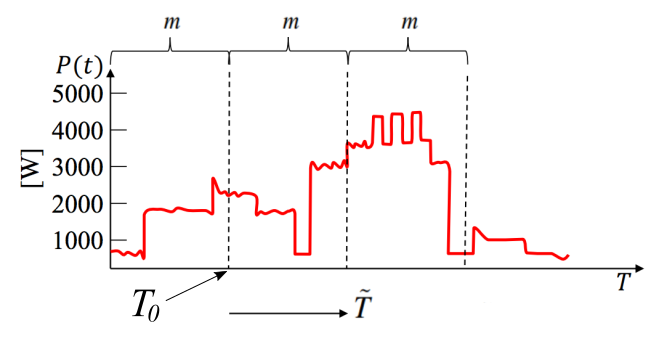
\includegraphics[width=1\columnwidth ]{windows2.png}
    \caption{New parameter $T_0$ necessary for creating new constraints to fix the sequence of states}
    \label{example}
\end{figure}


In Fig.~\ref{example}, power state $P_2(t)$ should be ON only if the power state $P_1(t)$ has finished. Likewise, we could also fix the power state $P_3(t)$ to be ON only if $P_2(t)$ has finished. The goal is to include a constraint that allows a specific power state to be activated only if a previous one (from the same appliance) has finished. To do so, two binary variables are used to determine the transition from a ON state to an OFF state, and vice versa. The two variables are called $up_i(t)$ (turned ON) and $dw_i(t)$ (turned OFF). Then, the linking constraints are given by \eqref{updw}--\eqref{updw2}.
%
%\vspace{-10pt}

\begin{equation} \label{updw}
    x_i(t) - x_i(t-1) = up_i(t) - dw_i(t) \quad \forall i \in S, t > T_0
\end{equation}


\begin{equation} \label{updw3}
    x_i(T_0) - X_i = up_i(t) - dw_i(t) \quad \forall i \in S, t = T_0
\end{equation}

\begin{equation} \label{updw2}
    up_i(t) + dw_i(t) \leq 1 \quad \forall i \in S, t \in \tilde{T}
\end{equation}

\noindent where $X_i$ saves the state $x_i(t)$ of the last time period of each window, necessary for the initialization of $x_i(t)$ in the next window. In constraint \eqref{updw}, $up_i(t)$ will be 1 only if the decision variable $x_i(t)$ makes a transition from 0 to 1, at time $t$. Likewise, $dw_i(t)$ will be 1 only if $x_i(t)$ makes a transition from 1 to 0, at time $t$. Next, \eqref{updw3} links the state transitions between windows. Finally, \eqref{updw2} prevents $up_i(t)$ and $dw_i(t)$ to be simultaneously 1.

%Now that we have these two variables, let's consider that we save the transition of states in a parameter called $\text{prev}_i$. In the Fig. \ref{example} we have for example in the washing machine that the value of $prev_2$ is 1 since we want to fix the second state to happen only after the first one. We can fix state transitions using the following constraint:

Using constraints \eqref{updw}--\eqref{updw2} and the parameter $\text{prev}_i$, we can now link the transition between two states using the additional equation in \eqref{state}.

\begin{equation} \label{state}
    up_i(t) = dw_{\text{prev}_i}(t) \quad \forall i \in S, t \in \tilde{T} \ | \ \text{prev}_i>0
\end{equation}

As an example, the state $i = 2$ of the washing machine in Fig.~\ref{example} can only change from OFF to ON (i.e., $up_2(t) = 1$) if the state $i = 1$ has change from ON to OFF (i.e., $dw_1 = 1$), at a given time $t$.

\subsection{Minimum Active Time}

One last hypothesis that is proposed in this paper is setting a minimum active time of a state. Parameter $MD_i$ in Fig.~\ref{example} establishes the minimum number of time samples in which the state $i$ should be kept activated. The set of constraints presented in \eqref{md1}--\eqref{md3} are proposed to carry out this process. 

\begin{equation}\label{md1}
    \sum_{k\ =\ T_0}^{G_i} \left[ 1 - x_i(k) \right] = 0 \quad \forall i \in S
\end{equation}

\begin{multline}\label{md2}
    \sum_{k\ =\ t}^{t+MD_i-1} x_i(k) \geq MD_i \left[ x_i(t) - x_i(t-1) \right] \\
    \forall i \in S, t \in G_i + T_0 \hdots T_f - {MD}_i + 1
\end{multline}

\begin{multline} \label{md3}
    \sum_{k\ =\ t}^{T_f} \left\{ x_i(k) - \left[ x_i(t) - x_i(t-1) \right] \right\} \geq 0 \\
    \forall i \in S, t \in T_f - MD_i + 2 \hdots T_f 
\end{multline}

Constraint \eqref{md1} activates a certain state that was already activated at the end of the previous window, but for less than $MD_i$ samples. Parameter $G_i$ is the number of periods in which the state $i$ must remain ON at the beginning of the window. It is calculated as $G_i = \min \left\{ T_f, \left[ MD_i - NP_i \right] X_i \right\}$. $NP_i$ is the number of time periods in which $i$ has been activated in the previous window, given by the equation \eqref{np}

\begin{equation} \label{np}
    NP_i = \sum_{k\ =\ T_f - MD_i + 2}^{T_f} { x_i(k) } \quad \forall i \in S
\end{equation}

Constraint \eqref{md2} forces $x_i(t)$ to be 1 for at least $MD_i$ time samples. Finally, constraint \eqref{md3} is used to represent the operation at the final portion of the window, when there are less than $MD_i$ samples available. It forces a given state $x_i(t)$ to be ON until the end of the window, only if it has been activated at any moment within this final interval. The size of $MD_i$ has as limit the length $m$ of the window, i.e, $MD_i \leq m$. 
As a side note, the set of equations presented in \eqref{overl}--\eqref{md3} are similar to models of the operation of thermal units in the unit commitment problem, proposed by authors in \cite{carrion2006}.

\section{Full Proposed Model}

The full proposed model is given by the Algorithm \ref{algorithm2}. As it will be illustrated in the next section, this kind of optimization problem can be solved with the help of standard convex mathematical optimization software. 

\begin{algorithm}[H]\label{algorithm2}
\SetAlgoLined
 \Repeat{$T_0$ > $T_f$}{

let  $\tilde{T} = \left\{T_{0}, \cdots, T_{0}+m \right\}$

solve
$$\min_{x_i(t)} \quad \sum_{t\ \in\ \tilde{T}} \delta_P(t) + \delta_Q(t)$$

s. t. 
\begin{center}
$(\ref{first_eq})$ ... $(\ref{md3})$
\end{center}

let $T_0 = T_0 +m$ + 1
 }
\caption{Proposed NILM using a window-based algorithm.}
\end{algorithm}

\vfill


\section{Summary}
- This chapter has presented a set of constraints for modeling the load signature, which are the main contributions of this work. 
- This chapter has expanded the classic NILM CO model for modeling load signatures in a computationally efficient way. 
- First, the classic CO problem was reformulated to a MILP problem. Next, a window based formulation was presented in order to decrease the computational burden. Then, constraints were introduced for modeling the load signature based on three features: power state, minimum time and sequence of states. As we will see in the next chapter, those features can be extracted from a model in both a supervised and unsupervised setting. 